\InputIfFileExists{ztex_doc-cfg.tex}{}{}
\documentclass[hyper, lang=cn]{ztex}
\usepackage{ztikz}
\ztexset{
  toc={
    column  = 2,
    title   = 总目录,
    stretch = 1.3
  }
}
\ztikzloadlib{basic, cache, gnuplot, python, wolfram, l3draw}
\usepackage{minted}
\definecolor{bg}{rgb}{0.95,0.95,0.95}
\fvset{gobble=0}
\setmonofont{Latin Modern Mono}
  [
    BoldFont=*,
    ItalicFont=* Slanted,
    BoldItalicFont=* Slanted,
    BoldFeatures={FakeBold=2},
    BoldItalicFeatures={FakeBold=2},
  ]
\setminted{
  bgcolor=bg,
  breaklines=true, 
  tabsize=2,
  breakanywhere=true,
  breaksymbolright=$\swarrow$,
  breakanywheresymbolpre=,
  breaksymbolleft=,
}
% important: avoid conflict with tikz externalize 'prefix' settings
\usepackage[most]{tcolorbox}
\tcbuselibrary{external}
\tcbsetforeverylayer{shield externalize} 
\newcounter{DocExample}
\tcbuselibrary{hooks}
\tcbuselibrary{minted}
\tcbset{listing engine=minted}
\def\mintLang{tex}
\DeclareTCBListing{DocExample}{!s!O{@@}}{
  enhanced, 
  breakable,
  segmentation style={white},
  arc=2pt, frame hidden, 
  enhanced jigsaw,
  opacityback=0, 
  sharp corners, 
  colframe=black, boxrule=.4pt,
  left=.5mm, right=1mm,
  top=0mm, bottom=0mm, 
  \IfBooleanTF{#1} 
    {text and listing}
    {listing only},
  minted language=\mintLang, 
  minted options = {  
    autogobble,
    escapeinside=#2,
    fontsize=\small,
  },
  before upper app={\begin{center}},
  after upper pre={\end{center}\vspace*{-2em}},
  % after pre={\newpage},
}
\AddToHook{env/tcolorbox/before}{
  \stepcounter{DocExample}
  \ifnum\value{subsection}=0
  \else
    \newpage
  \fi
  \subsection{案例 \theDocExample}
}


\title{\ztikz{} Examples}
\author{Eureka}
\date{\today}
\begin{document}
\maketitle
\thispagestyle{empty}
\MakeLinkTarget*{ztikz-toc} 
\pdfbookmark[1]{总目录}{ztikz-toc}
\tableofcontents
\newpage

\section{介绍}
本文档展示了 \ztikz{} 宏包中部分命令或环境的使用示例, 希望本文档可以帮助用户更好的掌握与使用 \ztikz{} 宏集.


\clearpage
\section{basic/gnuplot 库}
\begin{DocExample}*
\begin{tikzpicture}[yscale=6, xscale=3]
  \ShowGrid{(-2,0); (2,1)}
  % pdf
  \Plot[domain=-2:2,style=teal]{1/(sqrt(0.2)*sqrt(2*pi))*exp(-(x-0)**2/(2*0.2**2))}
  \Plot[domain=-2:2,style=orange]{1/(sqrt(0.5)*sqrt(2*pi))*exp(-(x-0)**2/(2*0.5**2))}
  \Plot[domain=-2:2,style=green]{1/(sqrt(1)*sqrt(2*pi))*exp(-(x-0)**2/(2*1**2))}
  % cdf
  \Plot[domain=-2:2,style=teal]{0.5*(1+erf((x-0)/(sqrt(0.2)*sqrt(2))))}
  \Plot[domain=-2:2,style=orange]{0.5*(1+erf((x-0)/(sqrt(0.5)*sqrt(2))))}
  \Plot[domain=-2:2,style=green]{0.5*(1+erf((x-0)/(sqrt(1)*sqrt(2))))}
  % annotate
  \ShowPoint[radius=0pt]{(-1, 0); (0, 0); (1, 0)}
    [$\mu-\sigma$; $\mu=0$; $\mu+\sigma$][below]
  \ShowPoint[radius=0pt]{(1, 0.8); (1, 0.6); (1, 0.4)}[
    \textcolor{red}{\rule[1pt]{8pt}{3pt}}\;$\sigma^2=0.2$;
    \textcolor{orange}{\rule[1pt]{8pt}{3pt}}\;$\sigma^2=0.5$;
    \textcolor{green}{\rule[1pt]{8pt}{3pt}}\;$\sigma^2=1$;
  ][right=2em]
  \ShowPoint[radius=0pt]
    {(-1, 0.8); (-1, 0.6)}
    [
      $\displaystyle y = \frac{1}{\sigma\sqrt{2\pi}}\mathrm{Exp}
        \{-\frac{(x-\mu)^2}{2\sigma^2}\}$;
      $y=\frac12\left(1+\mathrm{Erf}(\frac{x-\mu}{\sigma\sqrt{2}})\right)$
    ]
\end{tikzpicture}
\end{DocExample}


\begin{DocExample}*
\begin{tikzpicture}[>=Latex]
  \xAxis[-1][12] \yAxis[-1][7]
  \PlotPrecise{plot}{22}
  \Plot[
    domain=0.75:11, 
    style={red, thick, opacity=0},
    marker={type=ball, color=red}
  ]{2.5-1/x}
  \PlotPrecise{plot}{22}
  \Plot[
    domain=0.5:11.5, 
    style={red, thick, opacity=0},
    marker={type=ball, color=green}
  ]{3+1/x}
  \PlotPrecise*{contour}{40}
  \ContourPlot[domain=0:12;, style={dashed}]{y-2.5}
  \ContourPlot[domain=0:12;, style={dashed}]{y-3}
\end{tikzpicture}
\end{DocExample}


\begin{DocExample}*
\ExplSyntaxOn
\clist_new:N \l__color_clist
\clist_set:Nn \l__color_clist {red, orange, yellow, green, blue, purple, brown, black}
\newcommand{\colorItem}[1]{\clist_item:Nn \l__color_clist {#1}}
\def\fptoint#1{\fp_to_int:n {#1}}
\ExplSyntaxOff
\begin{tikzpicture}[scale=11, >=Latex, font=\small]
  % plot and annotate
  \node at (.55, 0.15) [left] {$f(x)=\frac{1}{n}\sin(n+5)x$};
  \foreach \i in {6, 7, 8, 9, 10, 11, 12, 13}{
    \Plot[
      domain=0:pi/3, 
      style=\colorItem{\fpeval{\i-5}}
    ]{\fpeval{1/\i}*sin(\fpeval{\i+5}*x)}
    \node[color=\colorItem{\fpeval{\i-5}}] 
      at (1, \fpeval{(\i-6)*0.03}) [right] {$n=\i$};
  }
  % axis draw
  \ShowAxis [
    tickStyle=above,    axisColor=gray,
    tickStart=-0.15,    tickEnd=0.18,
    mainStep=0.05,
    mainTickColor=gray, mainTickLabelPosition=left,
    mainTickLength=.5pt,axisRotate=90,
  ]{(-0.18, 0); (0.18, 0)}
  \ShowAxis [
    tickStyle=below,    axisColor=gray,
    tickStart=0,        tickEnd=1.22,
    mainStep=\fpeval{pi/18},
    mainTickColor=gray, subTickLength=0pt, 
    mainTickLength=.5pt, 
    mainTickLabel={\fptoint{\CurrentFp/(pi/18)*10}$^\circ$}
  ]{(0, 0); (1.25, -0)}
\end{tikzpicture}
\end{DocExample}


\begin{DocExample}*
\begin{tikzpicture}[>=Latex]
  \xAxis[0][10] \yAxis[-3.25][3.25]
  \Plot[domain=0:10]{2*sqrt(x)*cos(log(x))*sin(x)}
  \PlotPrecise{plot}{40}
  \Plot[
    domain=0:10, style={opacity=0}, 
    marker={type=*, color=red}
  ]{2*sqrt(x)*cos(log(x))*sin(x)}
  \BarPlot[x][
    fill=orange!35!white, 
    bar width=\fpeval{10/40}cm, 
    opacity=.75, very thin, draw=orange
  ]{\gnudata{2}}
\end{tikzpicture}
\end{DocExample}


\begin{DocExample}*
\begin{tikzpicture}[scale=.8, >=Latex]
  \ShowGrid[step=1, color=gray, opacity=.5]{(0, 0); (10, 10)}
  \xAxis[-1][10]  \yAxis[-1][10]
  \Plot[
    domain=0:10,
    style={red, jump mark right, very thick, xshift=2pt},
    marker={type=*, opacity=0}
  ]{floor(x)}
  \Plot[domain=0:10, style={dashed, blue}]{x}
  \Plot[domain=1:10, style={dashed, orange}]{x-1}
  \PlotPrecise{plot}{11}
  \Plot[
    domain=0:10,
    style={opacity=0, jump mark right},
    marker={type=o, color=blue}
  ]{x}
  \PlotPrecise{plot}{11}
  \Plot[
    domain=0:10,
    style={opacity=0, jump mark right},
    marker={type=*, color=red}
  ]{x-1}
  \ShowPoint[opacity=0]{(2, 9); (2, 8); (2, 7)}
    [$y=\lfloor x\rfloor$; $y=x$; $y=x-1$][right]
\end{tikzpicture}
\end{DocExample}


\begin{DocExample}*
\begin{tikzpicture}[>=Latex, font=\small]
  \clip (-6, -1) rectangle (3, 6);
  \ShowAxis{(-8, 0); (3, 0)}  \ShowAxis{(0, -1.5); (0, 6)}
  \Plot[domain=-8:5,    style={red}]     {exp(x)}
  \Plot[domain=-8:5,    style={blue}]    {exp(1)/4*(x+1)**2}
  \Plot[domain=-8:5,    style={green}]   {exp(1)*x + (x-1)**2}
  \Plot[domain=-8:5,    style={purple}]  {x**2 + 1}
  \Plot[domain=-8:0.95, style={gray}]    {1/(1-x)}
  \Plot[domain=-8:1.95, style={orange}]  {(2+x)/(2-x)}
  \Plot[domain=-8:5]                     {x+1}
  \Plot[domain=-8:8]                     {exp(1)*x}
  \ContourPlot[domain={0:2;-6:6}, style=dashed] {x-1}
  \ShowPoint[color=red, radius=1pt]{(-1, 0); (0, 1); (1, 2.71828)}
    [$A$; $B$; $C$][above left]
\end{tikzpicture}
\end{DocExample}



\begin{DocExample}*
\begin{tikzpicture}[>=Latex, font=\small]
  \clip (-2, -2) rectangle (10, 4);
  \ShowAxis{(-2, 0); (12, 0)} \ShowAxis{(0, -2); (0, 4)}
  \Plot[domain=-5:12, style={red}]     {log(x)}
  \Plot[domain=0:12,  style={blue}]    {(x-1)/x}
  \Plot[domain=0:12,  style={teal}]    {2*(x-1)/(x+1)}
  \Plot[domain=-1:12, style={purple}]  {6*(x-1)/(2*x+5)}
  \Plot[domain=-5:12, style={gray}]    {x/exp(1)}
  \Plot[domain=0.1:12,style={orange}]  {0.5*(x-1/x)}
  \Plot[domain=-5:12]                  {x-1}
  \Plot[domain=-5:12, style=green]     {x**2-x}
  \ContourPlot[domain={-5:12;-6:6}, style=dashed]{y-1}
  \ShowPoint[color=red, radius=1pt]{(1, 0);(2.71828, 1)}
    [$A$; $B$][above left]
\end{tikzpicture}
\end{DocExample}


\begin{DocExample}*
% https://texample.net/tikz/examples/polar-coordinates-template/
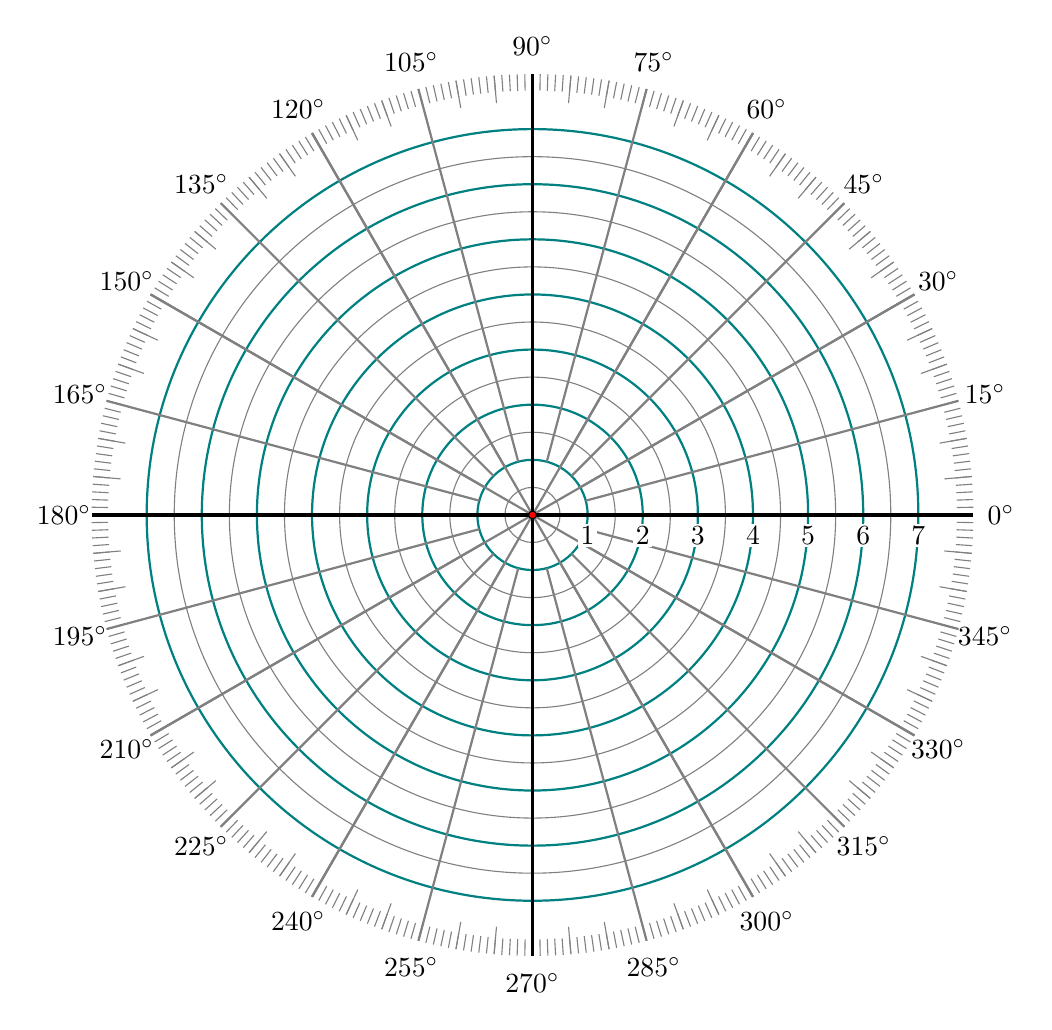
\begin{tikzpicture}[scale=.7]
  \foreach \r in {1, 2,...,7}     \draw[teal,thick] (0,0) circle (\r);    
  \foreach \r in {0.5, 1.5,...,7} \draw[gray, thin] (0,0) circle (\r);
  \foreach \a in {0, 1,...,359}   \draw[gray] (\a:7.7) -- (\a:8);
  \foreach \a in {0, 5,...,359}   \draw[gray] (\a:7.5) -- (\a:8);      
  \foreach \a in {0, 15,...,359}  \draw[thick,gray] (\a:1) -- (\a:8); 
  \foreach \a in {0, 30,...,359}  \draw[thick,gray] (0, 0) -- (\a:8);
  \foreach \r in {1, 2,...,7} 
    \draw (\r,0) node[inner sep=1pt,below=3pt,rectangle,fill=white] {$\r$};
  \foreach \a in {0, 90,...,359}  \draw[very thick] (0, 0) -- (\a:8);
  \foreach \a in {0, 15,...,359}  \draw (\a: 8.5) node {$\a^\circ$};
  \draw[fill=red] (0,0) circle(0.7mm);
  \PolarPlot[domain=0:2*pi, style={thick, orange}]{t}
\end{tikzpicture}
\end{DocExample}


\clearpage
% \def\mintLang{mathematica}
\section{wolfram 库}
\begin{DocExample}*
\begin{wolframGraphics}{wolframStroke}
fp1 = ContourPlot[
  x^2 + y^2 == 4, {x, -1.3, 0.6}, {y, -2.4, 3.2}, 
  AspectRatio->(2.4+3.2)/(1.3+0.6), ContourStyle->Red
];
fp2 = ContourPlot[
  x^2 + y^2 == 4, {x, -3, 3}, {y, -3, 3}, 
  AspectRatio->1, ContourStyle->RGBColor["#00C0A3"], 
  AxesOrigin->{0, 0}, Axes->True
];
fp3 = ContourPlot[
  {x^2 + y^2 == 4, x^2 + Sin[y] == 1},
  {x, -2.5, 2.5}, {y, -3, 3},
  ContourStyle->{
    {RGBColor["#00C0A3"], Thickness[0.01]},
    {RGBColor["#FF9671"], Thickness[0.01]}
  },
  AspectRatio->(3+3)/(2.5+2.5), AxesOrigin->{0,0},
  Axes->True, Frame->False,
  AxesStyle->Arrowheads[{0,0.01}]
]
FIGURE = Show[fp2, fp1, fp3];
\end{wolframGraphics}
\includegraphics[width=.5\linewidth]{\wolframOuputFile}
\end{DocExample}



\begin{DocExample}*
\begin{wolframGraphics}{wolfram2Dplot}
plotFunction[fun_, xlimits_, ylimits_] := ContourPlot[ 
  fun, xlimits, ylimits,
  ContourStyle->{
    RGBColor["#00C0A3"], 
    Thickness[0.004]
  },
  AspectRatio->((xlimits[[2]]//Abs) + (xlimits[[3]]//Abs))
              /((ylimits[[2]]//Abs) + (ylimits[[3]]//Abs)), 
  AxesOrigin->{0,0}, 
  Axes->True, Frame->False,
  AxesStyle->Arrowheads[{0, 0.03}],
  AxesLabel->{"x", "y"},
  PlotRange -> Full
]

xlimits = {x, -3, 6};
ylimits = {y, -4, 5};
fp1 = plotFunction[y==Sin[x], xlimits, ylimits];
fp2 = plotFunction[x^2/4 + y^2/3 == 5, {x, -5, 5}, {y, -5, 5}];
FIGURE = Show[fp2, fp1];
\end{wolframGraphics}
\includegraphics[width=.5\linewidth]{\wolframOuputFile}
\end{DocExample}



\begin{DocExample}*
\begin{wolframGraphics}{wolfram3DAxis}
(* 1. 定义一个产生箭头的命令 *)
arrow[start_, end_, type_] := Graphics3D[ 
  { type, 
    { Arrowheads[.02], Arrow[Tube[{start, end}, 0.06]]} 
  }, Boxed->False
];
(* 2. 创建三个坐标轴的箭头, 使用颜色进行区分 *)
xaxis = arrow[{-10, 0, 0}, {10, 0, 0}, Blue];
yaxis = arrow[{0, -10, 0}, {0, 10, 0}, Green];
zaxis = arrow[{0, 0, -10}, {0, 0, 10}, Red];
(* 3. 展示在同一坐标轴 *)
axis = {xaxis, yaxis, zaxis};
(* 4. 绘制一个函数由于测试 *)
fp4 = Plot3D[
  0.4*x + 0.2*Sin[y] + 0.2*x*y, 
  {x, -5, 7}, {y, -6, 4}, 
  ColorFunction->"Rainbow"
];
(* 5. 显示三维函数图像和坐标轴 *)
FIGURE = Show[axis, fp4]
\end{wolframGraphics}
\includegraphics[width=.5\linewidth]{\wolframOuputFile}
\end{DocExample}


\begin{DocExample}*
\begin{wolframGraphics}{wolfram3DParametric}
FIGURE = ParametricPlot3D[
  {1.16^v*Cos[v]*(1+Cos[u]), -1.16^v*Sin[v]*(1+Cos[u]), -2 1.16^v*(1+Sin[u])},
  {u, 0, 2*Pi}, {v, -15, 6},
  PlotStyle->{Opacity[0.6],Red},
  PlotRange->All, PlotPoints->25,
  Axes->False, Boxed->False
];
\end{wolframGraphics}
\includegraphics[width=.4\linewidth]{\wolframOuputFile}
\end{DocExample}


\begin{DocExample}*
\begin{wolframGraphics}{wolframLine-I}
FIGURE = NumberLinePlot[
  { Interval[{5, Infinity}], Interval[{2, 7}] }, 
  AxesStyle->Arrowheads[{0, 0.01}]
];
\end{wolframGraphics}
\edef\mmaOutputTmp{\wolframOuputFile}

\begin{wolframGraphics}{wolframLine-II}
fvec = VectorPlot[
  {1, x^2}, {x, -4, 4}, {y, -4, 4}, 
  AxesOrigin->{0, 0}, Axes->False, Frame->False
];
fp = Plot[
  1/3*x^3, {x, -2, 2}, PlotStyle->Red, 
  AxesStyle->Arrowheads[{0, 0.01}] 
];
FIGURE = Show[fp, fvec];
\end{wolframGraphics}
\includegraphics[width=.45\linewidth]{\mmaOutputTmp}\qquad
\includegraphics[width=.45\linewidth]{\wolframOuputFile}
\end{DocExample}


\begin{DocExample}*
\begin{wolframGraphics}{wolframHamiltonian}
g = RandomGraph[{20, 100}];
h = FindHamiltonianCycle[g];
FIGURE = HighlightGraph[g, Style[h, Directive[Thick, Red]]];
\end{wolframGraphics}
\edef\mmaOutputTmp{\wolframOuputFile}

\begin{wolframGraphics}{wolframStatistic}
FIGURE = BarChart[Flatten[Table[{i, j}, {i, 1, 4}, {j, 1, 3}], 1]];
\end{wolframGraphics}
\includegraphics[width=.45\linewidth]{\mmaOutputTmp}\qquad
\includegraphics[width=.45\linewidth]{\wolframOuputFile}
\end{DocExample}


\begin{DocExample}*
\begin{wolframGraphics}{wolfram2DBall}
xls = RandomInteger[{0, 20}, 80];
yls = RandomInteger[{0, 20}, 80];
xycoor = {xls, yls}//Transpose;
color = { RGBColor["#00A894"], RGBColor["#008896"], RGBColor["#006780"], RGBColor["#2F4858"], RGBColor["#70986B"]};
fp1 = Table[
  Graphics[{ color[[RandomInteger[{1, 5}]]], 
    Disk[xycoor[[i]], RandomReal[{0, 0.05}]*#1+RandomReal[{0, 0.05}]*#2&[xycoor[[i]][[1]], xycoor[[i]][[2]]]]
  }], {i, 1, 80}
];
fp2 = ListPlot[xycoor, AspectRatio->(Max[yls])/(Max[xls])];
FIGURE = Show[fp2, fp1];
\end{wolframGraphics}
\edef\mmaOutputTmp{\wolframOuputFile}

\begin{wolframGraphics}{wolfram3DBall}
FIGURE = Graphics3D[{
    Blue, Opacity[0.5], Sphere[{0.5, 0.5, 0}, 0.5],
    Blue, Opacity[0.5], Sphere[{-0.5, -0.5, 0}, 0.5],
    Blue, Opacity[0.5], Sphere[{0.5, -0.5, 0}, 0.5], 
    Blue, Opacity[0.5], Sphere[{-0.5, 0.5, 0}, 0.5],
    Blue, Opacity[0.5], Sphere[{0, 0, 0.5}, 0.5],
    Blue, Opacity[0.5], Sphere[{0, 0, -0.5}, 0.5],
    Green,Sphere[{0,0,0}, 0.75]
  }, Boxed->False
];
\end{wolframGraphics}
\includegraphics[width=.4\linewidth]{\mmaOutputTmp}\qquad
\includegraphics[width=.4\linewidth]{\wolframOuputFile}
\end{DocExample}


\clearpage
% \def\mintLang{python}
\section{python 库}
\begin{DocExample}*
\begin{pyfig}{pyfigExampleA}{pyfig-A.pdf}
# https://matplotlib.org/stable/gallery/lines_bars_and_markers/histogram_demo.html
import matplotlib
matplotlib.use('Agg')
import matplotlib.pyplot as plt
import numpy as np

np.random.seed(19680801)
n_bins = 10
x = np.random.randn(1000, 3)
fig, ((ax0, ax1), (ax2, ax3)) = plt.subplots(nrows=2, ncols=2)
colors = ['red', 'tan', 'lime']
ax0.hist(x, n_bins, density=True, histtype='bar', color=colors, label=colors)
ax0.legend(prop={'size': 10})
ax0.set_title('bars with legend')
ax1.hist(x, n_bins, density=True, histtype='bar', stacked=True)
ax1.set_title('stacked bar')
ax2.hist(x, n_bins, histtype='step', stacked=True, fill=False)
ax2.set_title('stack step (unfilled)')
x_multi = [np.random.randn(n) for n in [10000, 5000, 2000]]
ax3.hist(x_multi, n_bins, histtype='bar')
ax3.set_title('different sample sizes')
fig.tight_layout()
\end{pyfig}
\includegraphics[width=.7\linewidth]{\pyfigOutputFile}
\end{DocExample}



\begin{DocExample}*
\begin{pyfig}{pyfigExampleB}{pyfig-B.pdf}
# https://matplotlib.org/stable/gallery/mplot3d/stem3d_demo.html
import matplotlib
matplotlib.use('Agg')
import matplotlib.pyplot as plt
import numpy as np

theta = np.linspace(0, 2*np.pi)
x = np.cos(theta - np.pi/2)
y = np.sin(theta - np.pi/2)
z = theta

fig, ax = plt.subplots(subplot_kw=dict(projection='3d'))
ax.stem(x, y, z)
\end{pyfig}
\includegraphics[width=.75\linewidth]{\pyfigOutputFile}
\end{DocExample}


\begin{DocExample}*
\begin{pyfig}{pyfigExampleC}{pyfig-C.pdf}
# https://matplotlib.org/stable/gallery/mplot3d/voxels_numpy_logo.html
import matplotlib
matplotlib.use('Agg')
import matplotlib.pyplot as plt
import numpy as np

def explode(data):
  size = np.array(data.shape)*2
  data_e = np.zeros(size - 1, dtype=data.dtype)
  data_e[::2, ::2, ::2] = data
  return data_e

# build up the numpy logo
n_voxels = np.zeros((4, 3, 4), dtype=bool)
n_voxels[0, 0, :] = True
n_voxels[-1, 0, :] = True
n_voxels[1, 0, 2] = True
n_voxels[2, 0, 1] = True
facecolors = np.where(n_voxels, '#FFD65DC0', '#7A88CCC0')
edgecolors = np.where(n_voxels, '#BFAB6E', '#7D84A6')
filled = np.ones(n_voxels.shape)

# upscale the above voxel image, leaving gaps
filled_2 = explode(filled)
fcolors_2 = explode(facecolors)
ecolors_2 = explode(edgecolors)

# Shrink the gaps
x, y, z = np.indices(np.array(filled_2.shape) + 1).astype(float) // 2
x[0::2, :, :] += 0.05
y[:, 0::2, :] += 0.05
z[:, :, 0::2] += 0.05
x[1::2, :, :] += 0.95
y[:, 1::2, :] += 0.95
z[:, :, 1::2] += 0.95

ax = plt.figure().add_subplot(projection='3d')
ax.voxels(x, y, z, filled_2, facecolors=fcolors_2, edgecolors=ecolors_2)
ax.set_aspect('equal')
\end{pyfig}
\includegraphics[width=.75\linewidth]{\pyfigOutputFile}
\end{DocExample}


\clearpage
\section{l3draw 库}
\begin{DocExample}*
% union 
\begin{Zdraw}
  \zxscale {0.5}  \zyscale {0.5}
  \zcirc {2cm, 0}{2cm}   \zcirc {3.5cm, 0}{2cm}
  \zusepath[draw, clip]  \zfcolor {teal!50}
  \zrect {-10cm, -10cm}{10cm, 10cm}
  \zusepath[fill]
\end{Zdraw}
% intersection 
\begin{Zdraw}
  \zxscale {0.5} \zyscale {0.5}
  \zcirc {3.5cm, 0}{2cm} \zusepath[draw]
  \zcirc {2cm, 0}{2cm}   \zusepath[clip, draw]
  \zfcolor {orange}      \zcirc {3.5cm, 0}{2cm}
  \zusepath[fill]
\end{Zdraw}
% difference
\begin{Zdraw}
  \zxscale {0.5}       \zyscale {0.5}
  \zfevenodd           \zfcolor {pink}
  \zcirc {2cm, 0}{2cm} \zcirc {3.5cm, 0}{2cm}
  \zusepath[draw, fill]
\end{Zdraw}
\end{DocExample}


\begin{DocExample}*
\begin{Zdraw}
  % draw circle
  \zxscale {.5} \zyscale {.5}
  \zcirc {-2cm, 0}{2.5cm}
  \zcirc {2cm, 0}{2.5cm}
  \zcirc {0, -2*sqrt(3)cm}{2.5cm}
  % add text
  \znewtext   \texta
  \zsetvtext  \texta {6em}{$y=\alpha x + \beta$\\ Hello~ world}
  \zscaletext \texta {2}{2}
  \zputtext   \texta {hc}{b}{0, -7cm}
  \zusepath[draw]
\end{Zdraw}
\end{DocExample}


\begin{DocExample}*
\ExplSyntaxOn
% Data Source: https://tex.stackexchange.com/a/721052/294585
\ztool_read_file_as_seq:neN 
  {\c_false_bool}{gradient.data} 
  \l_tmpa_seq   % seq(without outer brace)={0, 0}, {0.03, 0.01}, ..., {3.14, 0}.
\cs_set:Npn \color_gradient:n #1 
  { \color_select:n {blue!#1!green} }
\cs_generate_variant:Nn \color_gradient:n {e}

% Draw those segments
\draw_begin: \draw_cap_round:
\draw_xvec:n {1cm, 0}
\draw_yvec:n {0, 1cm}
\draw_path_moveto:n {\draw_point_vec:nn {0.785}{0}}
\int_step_inline:nnn {2}{\fp_eval:n {\seq_count:N \l_tmpa_seq-1}}
  {
    \seq_set_split:Nne \l_tmpb_seq {,}{\seq_item:Nn \l_tmpa_seq {#1}} 
    \seq_set_split:Nne \l_tmpc_seq {,}{\seq_item:Nn \l_tmpa_seq {\fp_eval:n {#1+1}}} 
    \color_gradient:e {\fp_eval:n {#1*100/\seq_count:N \l_tmpa_seq}}
    \draw_path_moveto:n {
      \draw_point_vec:nn {\seq_item:Nn \l_tmpb_seq {1}}
        {\seq_item:Nn \l_tmpb_seq {2}}
    }
    \draw_path_lineto:n {
      \draw_point_vec:nn {\seq_item:Nn \l_tmpc_seq {1}}
        {\seq_item:Nn \l_tmpc_seq {2}}
    }
    \draw_path_use_clear:n {draw} 
  }
\draw_path_use_clear:n {draw} \draw_end:
\ExplSyntaxOff
\end{DocExample}
\end{document}